\section*{Apéndice I: Códigos en Matlab}

%\subsection*{Bisección}
\begin{figure*}[h!]
\centering
  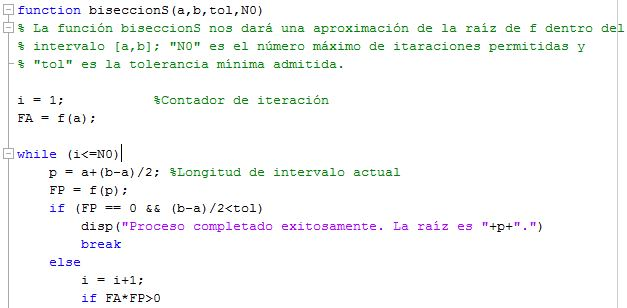
\includegraphics[width=1\textwidth]{BiseccionC1.JPG}
  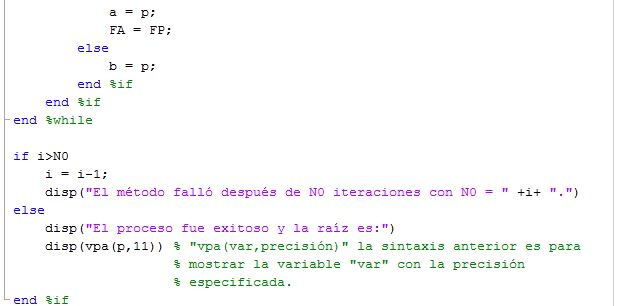
\includegraphics[width=1\textwidth]{BiseccionC2.JPG}
\end{figure*} 

%\subsection*{Falsa posición}
\begin{figure*}[h!]
\centering
  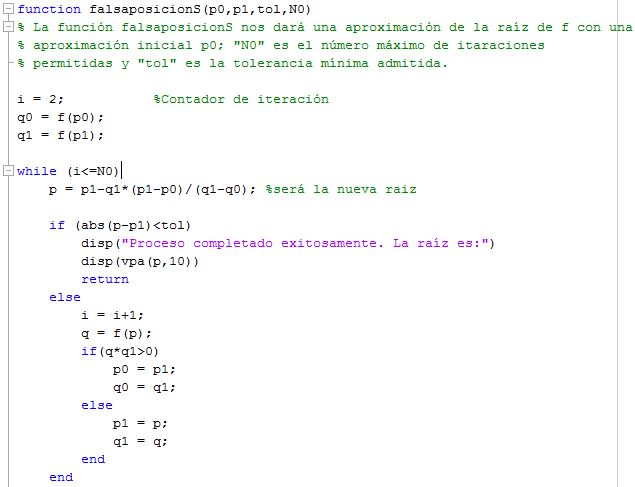
\includegraphics[width=1\textwidth]{FalsaC1.JPG}
  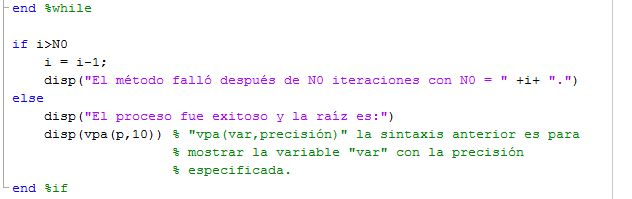
\includegraphics[width=1\textwidth]{FalsaC2.JPG}
\end{figure*} 

%\subsection*{Punto fijo}
\begin{figure*}[h!]
\centering
  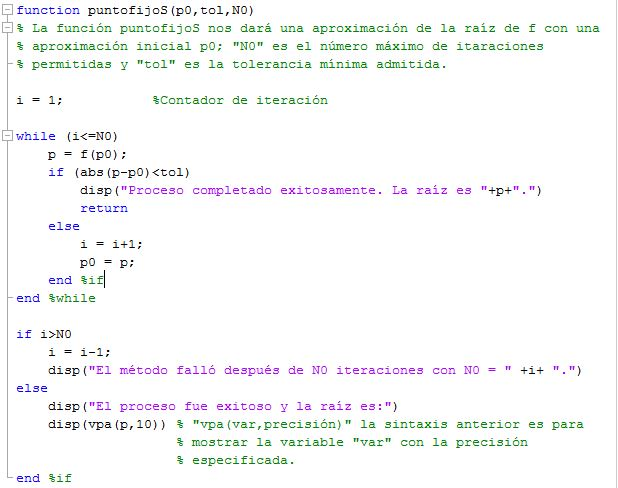
\includegraphics[width=1\textwidth]{PFijoC.JPG}
\end{figure*} 

%\subsection*{Newton}
\begin{figure*}[h!]
\centering
  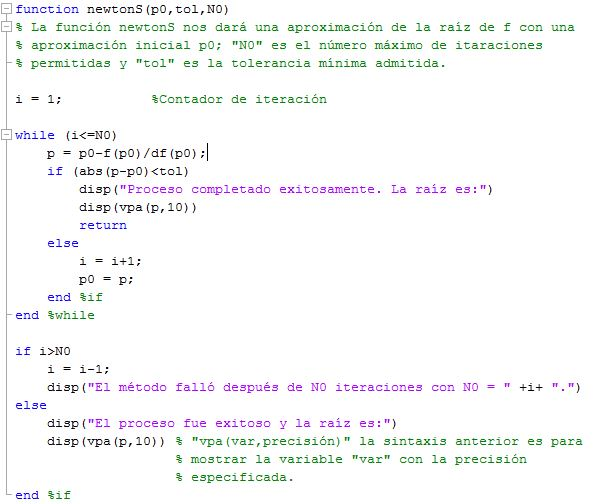
\includegraphics[width=1\textwidth]{NewtonC.JPG}
\end{figure*} 

%\subsection*{Newton en varias variables}
\begin{figure*}[h!]
\centering
  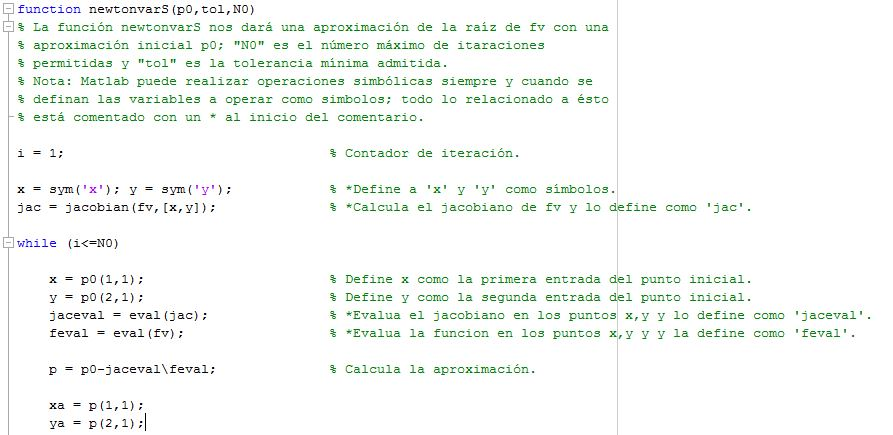
\includegraphics[width=1.2\textwidth]{NewtonVarC1.JPG}
  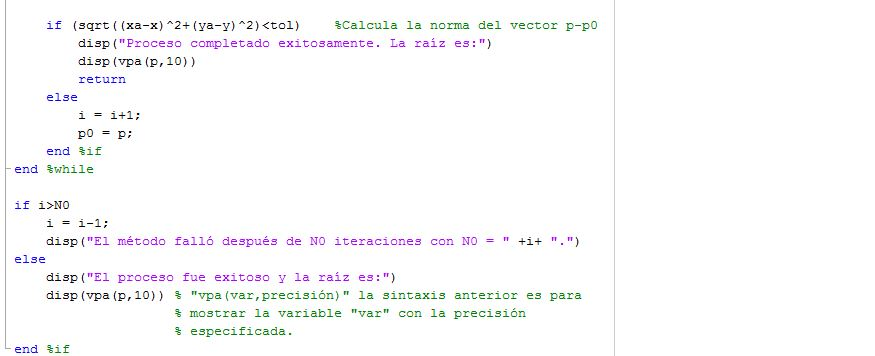
\includegraphics[width=1.2\textwidth]{NewtonVarC2.JPG}
\end{figure*} 